\documentclass{report}

\usepackage{amsmath}
\usepackage{amssymb}
\usepackage{bm}
\usepackage{graphicx}

\usepackage[linesnumbered, lined, boxed]{algorithm2e}
\RestyleAlgo{boxruled}

\DeclareMathOperator*{\argmax}{argmax}
\DeclareMathOperator*{\argmin}{argmin}

\usepackage[citestyle=authoryear, style=authoryear]{biblatex}
\addbibresource{paper.bib}

\usepackage{listings}
\lstset{frame = single,
breakatwhitespace=false,
breaklines=true,
numbersep=5pt,
showspaces=false,
showtabs=false,
tabsize=2,
basicstyle=\footnotesize}

\usepackage{geometry}
\geometry{margin=1.5in}

\author{Tom Wallace}

\title{STAT 672 Final Project: Stochastic Gradient Descent}

\begin{document}

\maketitle

\tableofcontents

\newpage

\chapter{Introduction}

\section{Organization}

This paper is divided into four sections. The remainder of this
\textbf{Introduction} section gives intuitive motivation for stochastic gradient
descent (SGD). The \textbf{Method and Theory} section more rigorously derives
SGD, outlines convergence properties, and reviews extensions to the basic
algorithm. The \textbf{Applications} sections highlights SGD's role in
statistical learning, including a simulation analysis to demonstrate SGD's utility
in large-$n$ settings. The \textbf{Conclusion} section summarizes
overall findings.

\section{Motivation}

SGD is an optimization algorithm commonly used for fitting coefficients
in statistical models, particularly in non-parametric and large-$n$ settings.
Before covering exactly how SGD works, we contextualize its advantages in these areas.

\subsection{Parametric vs. non-parametric approaches}

Consider a feature matrix $\bm{X}$ and outcome variable $\bm{Y}$, and the task
of fitting coefficients in a model to predict $Y_i$ based on $\bm{X}_i$. 
Assuming that particular model elements follow a
known statistical distribution aids the estimation of coefficients. 
For example, assumptions in ordinary least squares (OLS)
regression---assumptions that readers almost certainly are familiar with and so will not be
repeated here---allow a closed form solution, $\hat{\bm{\beta}} = (\bm{X}'\bm{X})^{-1}\bm{X}'\bm{Y}$.

Even if a parametric model does not have a closed-form solution, the parametric
assumption allows some useful optimization techniques. Consider logistic
regression. The maximum likelihood estimator (MLE) approach for estimating
coefficients leads to a system of $D$ equations. This system of
equations typically is numerically solved using the iterative Newton-Raphson
algorithm:

$$
\hat{\bm{\beta}}^{(t+1)} = \hat{\bm{\beta}}^{(t)} -
\bm{H}^{-1}(\hat{\bm{\beta}}^{(t)})\bm{J}(\hat{\bm{\beta}}^{(t)})
$$

$(t)$ refers to a particular iteration, $\bm{J}$ is the Jacobian of the
log likelihood function $l$,
and $\bm{H}$ is the Hessian of $l$. The practicality of Newton-Raphson thus depends on whether it is convenient to
find $\bm{J}$ and in particular $\bm{H}$. It is convenient for logistic regression
because parametric and independent-and-identically-distributed (IID) assumptions
mean $l$ is a simple sum of the log probability distribution
function (PDF) for each observation. We ``know'' (assume) the form of this PDF and so are
confident that the second derivative exists and is not onerous.
In non-parametric settings, we often cannot be so certain and face the possibility of
$\bm{H}$ being non-existent or cumbersome.

The need to conduct optimization in non-parametric settings is a chief
motivation for gradient descent (GD), of which SGD is a variant. SGD does not require any parametric assumptions. 
In its most basic form, SGD only requires finding the gradient (though some extensions
do need the Hessian or an approximation to it). 
SGD thus is well-suited for supervised and unsupervised statistical
learning, where parametric assumptions often are not made and 
Newton-Raphson and other second-order methods often are undesirable. 

\subsection{Computational complexity}

How an optimization technique scales with sample size $n$ is another important
consideration. It is little comfort if a method reaches the correct solution but
requires an excessive amount of time to do so. ``Plain'' or
``batch'' GD requires evaluating the gradient for every observation,
every iteration, until the algorithm converges. For example, for a
dataset of $n=10^6$ that required 25 iterations to converge, batch GD would require 
evaluating the gradient $25 \times 10^6$ times. This scaling with
$n$ can cause untenably long computation time. Similarly, note that if the
Jacobian of some function has $D$ elements, the Hessian will have $D^2$. In
high-dimensional settings, this too can be computationally intractable.

In contrast, SGD evaluates the gradient for only a single randomly chosen observation per iteration. This
approach means convergence is ``noisier'' and hence requires more iterations to
converge, but each iteration is less compute-intensive and so can be done
faster. SGD thus scales more favorably with $n$ than does GD and so is
useful for large-$n$ applications.

\chapter{Method and theory}

\section{Basic form}

Suppose we want to minimize a function $f: \mathbb{R}^D \to \mathbb{R}$. 

\begin{equation}
	\min_w f(w)
\end{equation}

$f$ takes as input $w \in \mathbb{R}^D$. Assume
that $f$ is convex and differentiable, i.e. we can compute its gradient with
respect to $w$, $\nabla f(w)$. The optimal $w$, i.e. that which minimizes (2.1),
is denoted $\tilde{w}$. We are willing to settle for a close approximation
$\hat{w}$. The iterative GD algorithm for finding $\hat{w}$ is:

\begin{equation}
	w^{(t+1)} = w^{(t)} - \gamma \nabla f(w^{(t)})
\end{equation}

$t$ refers to a particular iteration. Assume that we have supplied an initial
starting guess $w^{(0)}$. $\gamma$ refers to step size (also called
learning rate). Assume for now that $\gamma$ is fixed. The GD algorithm iterates
until some stop condition is met. This may be a fixed number of iterations, or
that the quality of approximation meets some predefined threshold. 
A common stopping condition is when the L2 norm of the gradient
is less than some arbitrarily small constant. Obviously, the smaller the
constant, the closer $\hat{w}$ will be to $\tilde{w}$.

\begin{equation}
	||\nabla f(w^{(t)})||_2 \leq \epsilon
\end{equation}

Consider a modified situation. Suppose $f$ now takes two arguments, $w$ and $X
\in \mathbb{R}^D$. $f : \mathbb{R}^D \times \mathbb{R}^D \rightarrow
\mathbb{R}$. We have $n$ observations of $X$, and denote by
$\bm{X}_{n \times D}$ the matrix of these observations, with $X_i$ being a
row in that matrix. We apply $f$ over all observations, i.e. $\frac{1}{n} \sum_{i=1}^n f(w, X_i)$. Our new
problem is:

\begin{equation}
	\min_w  \frac{1}{n} \sum_{i=1}^n f(w, X_i)
\end{equation}

We could apply the GD algorithm above to find $\hat{w}$.

\begin{equation}
	w^{(t+1)} = w^{(t)} - \gamma \frac{1}{n} \sum_{i=1}^n \nabla f(w^{(t)},
	X_i)
\end{equation}

But, note that doing so requires evaluating the gradient at every single
observation $i \leq n$. This may be computationally intractable for large $n$
and high-dimensional $D$. The innovation of SGD is to instead evaluate only a
single randomly-chosen $i$ at each iteration $t$.

\begin{equation}
	w^{(t+1)} = w^{(t)} - \gamma \nabla f(w^{(t)}, X_i)
\end{equation}

As it turns out, SGD asymptotically converges to $\tilde{w}$ and does so in a computationally
advantageous way compared to GD.

\section{Key properties}

\subsection{Correctness}

This section gives intuition and partial proof for why SGD converges to
$\tilde{w}$.

Intuitively, our assumption that $f$ is convex means that there is one critical
point and it is the global minimum. Basic calculus tells us that this critical
point is located where $f'=0$ (in one dimension) or $\nabla f = 0$ (in higher
dimensions). So our task is to search in the space of $f$ for that point. We
start with some initial guess $w^{(0)}$, and every iteration, move ``down'' the
gradient in search of zero. Every iteration, we check if the gradient is equal
to 0; if not, we keep moving ``down.'' If the gradient is arbitrarily close to
zero, then we have found the critical point, which must be the value of $w$ that
minimizes $f$ and hence is $\tilde{w}$ (or at least a close approximation to it).

For a more formal proof---following that of \cite{tibs_notes}---assume (in addition to previously stated assumptions
that $f$ is convex and differentiable) that the gradient of $f$ is Lipschitz-continuous
with constant $L$, i.e. that $||\nabla f(x) - \nabla f(y)||_2 \leq L||x-y||_2$
for any $x, y$. This implies that $\nabla^2 f(w) - LI$ is a negative
semi-definite matrix. We perform a quadratic expansion of $f$ around $f(x)$ and
obtain the following inequality:
$$
f(y) \leq f(x) + \nabla f(x)^T(y-x) + \frac{1}{2}\nabla^2 f(x)||y-x||_2^2
$$
\begin{equation}
	\leq f(x) + \nabla f(x)^T(y-x) + \frac{1}{2}L||y-x||_2^2
\end{equation}

Now, suppose we use the GD algorithm presented in (2.2) with $\gamma \leq
\frac{1}{L}$. Denote $x^+ = x - \gamma \nabla
f(x)$ and substitute $x^+$ in for $y$:

$$ f(x^+) \leq f(x) + \nabla f(x)^T(x^+ - x) + \frac{1}{2}L||x^+ - x||_2^2 $$
$$ = f(x) + \nabla f(x)^T(x - \gamma \nabla f(x) - x) + \frac{1}{2}L||x - \gamma \nabla f(x) - x||_2^2 $$
$$ = f(x) - \nabla f(x)^T \gamma \nabla f(x)  + \frac{1}{2}L||\gamma \nabla f(x)||_2^2 $$
$$ = f(x) - \gamma||\nabla f(x)||_2^2 + \frac{1}{2} L \gamma^2||\nabla f(x)||_2^2$$
\begin{equation}
= f(x) - (1 - \frac{1}{2}L\gamma)\gamma||\nabla f(x)||_2^2 
\end{equation}

We have defined $\gamma \leq \frac{1}{L}$. This implies:
$$
-(1 - \frac{1}{2}L \gamma) = \frac{1}{2}L \gamma - 1
\leq \frac{1}{2}L\frac{1}{L} - 1
= \frac{1}{2} - 1
= - \frac{1}{2}
$$

Returning to (2.8), we obtain:

\begin{equation}
f(x^+) \leq f(x) - \frac{1}{2}\gamma||\nabla f(x)||_2^2
\end{equation}

A squared L2 norm will always be positive unless its content is
0, and we have defined $\gamma$ to be positive, so $\frac{1}{2} \gamma||\nabla f(x)||_2^2$ will always be positive unless the
gradient is equal to zero. So, (2.9) implies that GD results in a strictly
decreasing objective function value until it reaches the point where the
gradient equals zero, which is the optimal value. A key caveat is an
appropriately chosen $\gamma$, a point covered in more detail later.

The above proof is for GD. Proof is not given for why SGD also
converges to the optimal value. Informally, we can note that the above proof
says given infinite $t$ and appropriate $\gamma$, the iterative algorithm will
always converge to the optimal value. SGD is doing the same thing as GD, 
just with a single observation per iteration 
rather than the entire dataset per iteration. Since SGD is using less information
per iteration, we would expect the convergence to require more iterations. But
per (2.9) we expect it to \textit{eventually} arrive at the optimal solution.
If so, the difference between GD and SGD must then primarily revolve
around convergence speed, not the final value that is converged to.

\subsection{Speed}

Table 2.1---a simplified version of that in \cite{bottou2010large}---illustrates
the computational advantages of SGD over GD. As shown in row 1, because SGD uses
less information per iteration than GD, it requires more iterations to achieve
fixed degree of accuracy $\rho$.
However, row 2 shows that because GD computes the gradient for every observation every iteration,
while SGD only does so for a single randomly observation, GD's time per
iteration scales linearly with $n$ while SGD's is a constant. Thus, we conclude
that SGD's time to
reach accuracy $\rho$ scales only with $\rho$, while GD's scales with both
$\rho$ and---crucially---linearly with $n$. So, the larger $n$ grows, the larger
SGD's computational advantage over GD.

\begin{table}[h]
	\centering
	\caption{Asymptotic comparison of GD and SGD}
	\begin{tabular}{|l l l|}
		\hline
		& \textbf{GD} & \textbf{SGD} \\
		Iterations to accuracy $\rho$ & $\log \frac{1}{\rho}$ & $\frac{1}{\rho}$ \\
		Time per iteration & $n$ & 1 \\
		Time to accuracy $\rho$ & $n \log \frac{1}{p}$ & $\frac{1}{\rho}$ \\
		\hline
	\end{tabular}
\end{table}

Figure 2.1 visually compares SGD's convergence to that of GD (and
mini-batch gradient descent, a variation addressed later in this
paper).\footnote{Image taken from www.towardsdatascience.com} The
path of SGD's convergence is very squiggly, reflecting the extra variation
introduced by only using a single observation per iteration. The path of GD's
convergence is much smoother, reflecting the use of all observations per
iteration.

\begin{figure}[t]
	\centering
	\caption{Convergence}
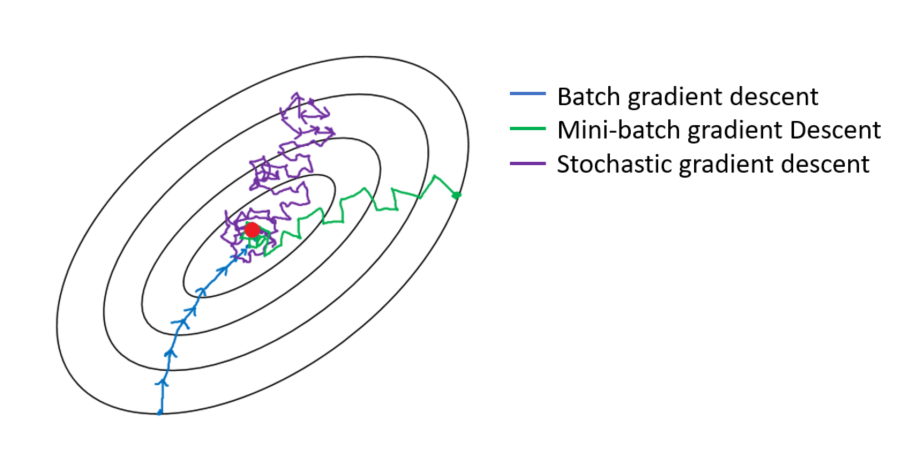
\includegraphics[scale=0.3]{img}
\end{figure}

\section{Extensions}

The basic SGD algorithm has been extended in many different ways. The popularity of
the algorithm disallows a comprehensive treatment of all
developments. This sub-section covers some of the more important
ones.


\subsection{Step size}

Much depends on
an appropriately chosen step size $\gamma$. If $\gamma$ is too small, gradient
descent may
take an excessively long time to run (since we are only moving a small distance
``down'' the gradient every iteration); if $\gamma$ is too large, then an
iteration's step may ``overshoot'' the critical point.
An entire literature has developed around the best way to select $\gamma$. The
central insight that is common to most $\gamma$-selection methods is to treat it
as a time-indexed rather than fixed hyperparameter, i.e., $\gamma^{(t)}$ rather
than $\gamma$. Ideally we would like $\gamma^{(t)}$ to be large when far away
from the critical point (so as to increase speed of convergence) and to be small
when close to the critical point (so as to avoid overshooting).

Line search is one method for computing step size. As described in
\cite{boyd2004convex}, there are two main variants: \textit{exact} and
\textit{backtracking}. In exact line search, $\gamma^{(t)}$ is chosen to minimize $f$
along the ray $\{x + \gamma^{(t)} \Delta x\}$, where $\gamma^{(t)} \in \mathbb{R}^+)$ and
$\Delta x$ is the descent direction determined by SGD:
\begin{equation}
	\gamma^{(t)} = \argmin_{s \geq 0} f(x + s\Delta x)
\end{equation}
This is an optimization problem in and of itself, and
so it can be computationally impractical to add this burden in addition to the
``main'' problem we are trying to solve using SGD. \textit{Backtracking} is an iterative approximation method that is
computationally lighter. The backtracking algorithm takes two hyper-parameters
$\alpha \in (0, 0.5)$ and $\beta \in (0, 1)$. It starts with an initial guess of
$s^{(0)} = 1$, and then for every iteration $t$, updates $s := \beta t$. The
algorithm stops when $f(x + s \Delta x) \leq f(x) + \alpha s \Delta f(x)^T
\Delta x$, and the final value of $s$ is taken as $\gamma^{(t)}$. 

\cite{bottou2012stochastic} advocates using learning rates of the form
$\gamma^{(t)} = \gamma^{(0)}(1 + \gamma^{(0)}\lambda t)^{-1}$. When the Hessian
$H$ of $f$ is strictly positive, using $\gamma^{(t)} =
(\lambda_{\mathrm{min}}t)^{-1}$, where $\lambda_{\mathrm{min}}$ is the smallest
eigenvalue of $H$, produces the best convergence speed. Note that $
(\lambda_{\mathrm{min}}t)^{-1}$ decreases asymptotically with $t$, matching our intuition
about larger step sizes in early iterations and smaller step sizes in later
iterations. However, simply using $\gamma^{(t)} =
(\lambda_{\mathrm{min}}t)^{-1}$ can produce \textit{too} large of steps in early
iterations. Hence, it often works better to start with some reasonable initial
estimate $\gamma^{(0)}$ that then decays in the fashion of
$(\lambda_{\mathrm{min}}t)^{-1}$. By definition, ``reasonable'' is more of a judgment
call than a mathematical statement: Bottou provides some heuristics for creating
such an estimate of $\gamma^{(0)}$.

\subsection{Momentum and acceleration}

In our set-up of SGD, we stipulated that the objective function is
convex. However, SGD is widely used in applications---most prominently, neural
networks and deep
learning---where this assumption is not
always true. In such settings, it is
possible that there are multiple local minima, and/or that there are areas where
the surface curves much more steeply in one dimension than another. The challenge for SGD is
how to avoid getting ``stuck'' in these local ravines and continue iterating
until the true global minimum is achieved. Even if there is no pathological
curvature, incorporating information about the local topology may result in more
efficient algorithms and faster convergence.

Momentum---also called acceleration---is a common modification of GD. As outlined in
\cite{rumelhart1986general} and 
\cite{qian1999momentum}, we add a new acceleration term to the familiar GD
equation. Let $z^{(t+1)} = \alpha z^{(t)} + \nabla f(w^{(t)})$. GD with
momentum then is:

\begin{equation}
	w^{(t+1)} = w^{(t)} - \gamma z^{(t+1)}
\end{equation}

Now, the weight vector obtained for the current timestep depends both on the
current gradient \textit{and the update of the previous time-step}, with the
acceleration parameter $\alpha$ governing how much weight is given to the
previous time-step. 
This formulation leads to momentum: dimensions whose
gradients point in the same direction have proportionally greater updates, while
dimensions whose gradients exhibit strong curvature have proportionally
lesser updates. The effect is to help stop SGD from oscillating in ravines and
speed up convergence. There are many variations on acceleration, including
Nesterov accelerated gradient (NAG) (\cite{nesterov}), Adam
(\cite{kingma2014adam}), AdaGrad
(\cite{duchi2011adaptive}), and AdaDelta (\cite{zeiler2012adadelta}).

\subsection{Averaging}

Averaged SGD (ASGD)---proposed in
\cite{polyak1992acceleration}---is another variation. Typically, we consider
$\hat{w}$ to be the final iteration
of SGD, when some stop condition is met. For example, in a situation where we
run $N$ iterations, $\hat{w} = w^{(N)}$. In ASGD, we consider $\hat{w}$ 
the average across all iterations.

\begin{equation}
	\hat{w} = \bar{w} = \frac{1}{N} \sum_{t=1}^N w^{(t)}
\end{equation}

The value proposition of ASGD is that sometimes SGD will oscillate around the
optimal solution. By taking the average across all updates, ASGD reduces this
noise and is likely to give a solution closer to the optimum. More sophisticated
versions of ASGD have been proposed in 
\cite{zhang2004solving}
and 
\cite{xu2011towards}. 

\subsection{Mini-batch}

Mini-batch gradient descent (MGD) is a mid-point between batch
and stochastic gradient descent: it uses more than one but less than all
observations per iteration. Suppose we have $n$ observations and divide them
into $m$ groups called mini-batches, each of equal size $b=\frac{n}{m}$. Now, at
every iteration $t$, randomly pick one of the mini-batches (all are equally
likely to be chosen). For that mini-batch:

\begin{equation}
	w^{(t+1)} = w^{(t)} - \gamma \frac{1}{b} \sum_{i=1}^b \nabla f(w^{(t)})
\end{equation}

MGD iterates with $t$ and converges to $\hat{w}$ in the normal manner. Every
update, a new $b$ is randomly chosen and the above algorithm iterated. 
\cite{dekel2012optimal} and \cite{li2014efficient} analyze MGD's speed of
convergence and suggest that has some advantageous qualities for
parallelization, a topic that is explained in more depth in the following
subsection.

\subsection{Parallelization}

SGD is common in large-$n$ applications. Thus,
even though SGD is a computational improvement over batch GD, there has been
interest in whether SGD can be made even faster via parallelization.
\cite{zinkevich2010parallelized} present a technique for doing so. Though backed
by very technical proofs, the actual algorithm is simple. Suppose we have $N$ processors. We seek to
use SGD to estimate $w$ across $n$ observations with fixed learning rate
$\gamma$ for fixed number of steps $T$.

\medskip

\begin{algorithm}[H]
	Define $T = \frac{n}{N}$\;

	Randomly partition examples, giving $T$ to each machine;\

	\ForAll{$i \in \{1 \ldots N\}$}{
		Randomly shuffle data on machine $i$\;

		Initialize $w^{i, (0)}=0$\;

		\ForAll{$t \in \{1 \ldots T\}$}{
			
	$w^{i, (t+1)} = w^{i, (t)} - \gamma \nabla f(w^{i, (t)})$ \;
			}
		}
	Aggregate from all computers: $\bar{w} = \frac{1}{N} \sum_{i=1}^{N}
	w^{i, (T)}$ \;

	\Return{$\bar{w}$}

	\caption{Parallel SGD}
\end{algorithm}

\medskip

Zinkevich et al. show that this algorithm has a number of desirable properties.
It requires no communication between machines until the end; asymptotically, the
error approaches zero; and, the amount of time required is independent of the number of
examples. Further improvements have been proposed e.g., the Hogwild algorithm
presented in \cite{recht2011hogwild}.

\chapter{Applications}

In theory, SGD is topic-agnostic and so can be used in many different areas of optimization. In
practice, SGD is overwhelmingly popular in the statistical learning
field for estimating weight coefficients in predictive models. 

\section{SGD and statistical learning}

Consider a typical supervised classification problem. We have
feature matrix $\bm{X}_{n \times D}$ ($n$ observations and $D$
features) and labels $\bm{Y}_{n \times 1}, Y_i \in \{-1, 1\}$. The goal is to
predict an observation's label $Y_i$ using that observation's features
$\bm{X}_i$. To emphasize the utility of SGD, suppose that both $n$ and $D$ are
very large.
We have a hypothesis class $\mathcal{F}$ of functions $f(\bm{w}, \bm{X}_i) \in \mathcal{F}$ parametrized by weight
vector $\bm{w}$. We have convex loss function $L(Y_i, f(\bm{w}, \bm{X}_i))$ that
expresses the cost of misclassification. 
We will consider the optimal function
that which minimizes empirical risk over all observations: $\frac{1}{n}
\sum_{i=1}^n L(Y_i, f(\bm{w}, \bm{X}_i))$.
Denote $\hat{\bm{w}}$ the weight coefficients of this optimal function. We thus
have:

\begin{equation}
	\hat{\bm{w}} = \argmin_{\bm{w}}\frac{1}{n} \sum_{i=1}^n L(Y_i, f(\bm{w}, \bm{X}_i))
\end{equation}

How shall we solve this optimization problem? Newton's method requires
calculating the Hessian, which will have $D^2$ entries; since $D$ is large,
this is inconvenient to compute. We could try batch gradient descent:

\begin{equation}
	\bm{w}^{(t+1)} = \bm{w}^{(t)} - \gamma \frac{1}{n}\sum_{i=1}^n
	\nabla_{\bm{w}} L(Y_i, f(\bm{w}^{(t)}, \bm{X}_i))
\end{equation}

But, in line with our analysis in section 2.2.2, batch GD requires evaluating
the gradient over every observation $i \leq n$ for every iteration $t$. Since we have defined $n$ to be
large, this is computationally inconvenient. Rather, we use SGD to evaluate only
a single randomly chosen observation per iteration.

\begin{equation}
	\bm{w}^{(t+1)} = \bm{w}^{(t)} - \nabla_{\bm{w}} L(Y_i, f(\bm{w}^{(t)}, \bm{X}_i))
\end{equation}

Per previous analyses we know that this approach will converge to an arbitrarily
good answer (if certain assumptions are met); will converge to that arbitrary
degree of precision in less time than plain gradient descent; does not
necessarily require computing the Hessian; and can be parallelized across many
machines. These attractive qualities make SGD well-represented in almost all areas of
machine learning. In the following subsection, we take a closer look at one
particularly prominent application, support vector machines.

\subsection{Support vector machines}

Originally proposed by \cite{boser1992training} and \cite{cortes1995support}, support vector machines (SVM)
are among the best supervised learning algorithms. Here we set up the SVM
optimization
problem and then show how SGD can be used to solve it.

Suppose we have labels $\bm{Y}$ with $Y_i \in \{-1,1\}$ and features $\bm{X}_{n
\times D}$, corresponding to $n$ observations and $D$ features.
We want to construct a decision hyperplane 
$\langle \bm{w}, \bm{X} \rangle + w_0= 0$. $\bm{w}$ is
a weight vector that we apply to $\bm{X}$. If for a particular observation $i$
$\langle \bm{w}, \bm{X}_i \rangle + w_0 < 0$, we
classify $Y_i=-1$. Similarly, if $\langle \bm{w}, \bm{X}_i \rangle + w_0 > 0$, we
classify $Y_i = 1$. We introduce slack variables $\xi_i$ to allow some
violation of the margin, as well as a cost parameter $C$ to control them. The
primal soft-margin SVM problem thus is:

\begin{equation}
	\min_{\bm{w} \in \mathbb{R}^D, w_0 \in \mathbb{R}, \bm{\xi} \in \mathbb{R}^n} 
	\frac{1}{2} ||\bm{w}||^2 + C \frac{1}{n} \sum_{i=1}^n \xi_i
\end{equation}
$$
s.t. \quad Y_i(\langle \bm{w}, \bm{X}_i \rangle + w_0) \geq 1 - \xi_i 
$$
$$
\quad \xi_i \geq 0 
$$

This problem can be recharacterized through the lens of empirical risk
minimization. Suppose we obtain an optimal answer $\bm{w}^*, w_0^*, \bm{\xi}^*$. 
Then:

$$
\xi_i^* = \max(0, 1 - Y_i(\langle \bm{w}, \bm{X}_i \rangle + w_0)) 
$$

We now can recharacterize the problem as:

$$
\min_{\bm{w}, w_0} C \frac{1}{n} \sum_{i=1}^n \left[ \max(0, 1 - Y_i(\langle \bm{w},
\bm{X}_i \rangle +
w_0)) + \frac{1}{2}||\bm{w}||^2 \right]
$$

This is equivalent to:

\begin{equation}
\min_{f \in \mathcal{F}} \frac{1}{n} \sum_{i=1}^n \left[ L(Y_i, \bm{w},
	\bm{X}_i) + \frac{\lambda}{2}
||\bm{w}||^2 \right]
\end{equation}

Where $\mathcal{F}$ is the linear hypothesis class, $L$ is the hinge loss

$$
L_{\mathrm{hinge}}(Y_i, \bm{w}, \bm{X}_i) = \max(0, 1 - Y_i
f(\bm{w}, \bm{X}_i))
$$
$$
f(\bm{w}, \bm{X}_i) = \bm{w}^T\bm{X}_i + w_0
$$

and
$\lambda=\frac{1}{2C}$. We use $\frac{\lambda}{2}$ for reasons of
convenience. This problem could solved using the Lagrangian dual, but SGD is a
popular method to solve the primal formulation given here. First note
that the hinge loss function is not differentiable. We must use a sub-gradient:

\begin{equation}
	\frac{\partial L}{\partial \bm{w}} = 
	\begin{cases}
		-Y_i \bm{X}_i \quad \mathrm{if} \hspace{0.2em} Y_if(\bm{w}, \bm{X}_i) < 1\\
		0 \quad \mathrm{otherwise} \\
	\end{cases}
\end{equation}

The basic batch GD approach

$$
	\bm{w}^{(t+1)} = \bm{w}^{(t)} - \gamma \frac{1}{n} \sum_{i=1}^n
	\nabla_{\bm{w}} \left[ L(Y_i, \bm{w},
	\bm{X}_i) + \frac{\lambda}{2}
||\bm{w}||^2\right]
$$

$$
	= \bm{w}^{(t)} - \gamma \frac{1}{n} \sum_{i=1}^n
	 \left[ L\nabla_{\bm{w}} (Y_i, \bm{w},
	\bm{X}_i) + \lambda \bm{w} \right]
$$
thus becomes
\begin{equation}
	\bm{w}^{(t+1)} = 
	\begin{cases}
		\bm{w}^{(t)} - \gamma \frac{1}{n} \sum_{i=1}^n
		\left[
			\lambda \bm{w}^{(t)} - Y_i\bm{X}_i
		\right]
		\quad \mathrm{if} \hspace{0.2em} Y_if(\bm{w}^{(t)}, \bm{X}_i) < 1 \\

		\bm{w}^{(t)} - \gamma \frac{1}{n} \sum_{i=1}^n
		\lambda \bm{w}^{(t)} 
		\quad \textrm{otherwise} \\

	\end{cases}
\end{equation}

As previously discussed, batch GD is computationally expensive and
so for large $n$ we prefer SGD, selecting only a single random
observation per iteration.

\begin{equation}
	\bm{w}^{(t+1)} = 
	\begin{cases}
		\bm{w}^{(t)} - \gamma 
		\left(
			\lambda \bm{w}^{(t)} - Y_i\bm{X}_i
		\right)
		\quad \mathrm{if} \hspace{0.2em} Y_if(\bm{w}^{(t)}, \bm{X}_i) < 1 \\

		\bm{w}^{(t)} - \gamma 
		\lambda \bm{w}^{(t)} 
		\quad \textrm{otherwise} \\

	\end{cases}
\end{equation}

There have been further efforts to improve SGD for the specific application of
SVM, most notably the Pegasos algorithm of \cite{shalev2011pegasos}.

\subsection{Neural networks and back-propagation}

Neural networks are another class of statistical learning
models for which SGD plays a fundamental role in estimating weights, in
particular through a process called back-propagation. Space
constraints disallow a detailed examination along the lines of that conducted
for SVM. This subsection aims only to note that SGD is widely used with neural
networks, and that this usage provides the practical motivation behind many of
the extensions to the SGD algorithm covered in Section 2.3. This is not to say
that these techniques are \textit{solely} intended for neural networks---indeed,
many of them precede neural networks' current popularity---but
their utility for neural networks is part of why the relevant papers have
thousands of citations.

Neural networks
often use non-convex loss functions that have multiple local minima in
which SGD can get ``lost'' while searching for global minimum.
Acceleration and momentum (2.3.2) thus are required to achieve effective
training, particularly on ``deep'' networks with many hidden layers
(\cite{sutskever2013importance}). Neural networks are
often extremely complex and high-dimensional and hence require enormous training
data (\cite{lecun2015deep}); hence, speeding up computation via parallelization
(2.3.5) or GPU computing is common. 

\section{Simulation case study}

Simulation provides an example of the computational advantages of SGD. 
Suppose we have one-dimensional feature matrix $\bm{X}$ with $X_i \sim N(0, 1)$ 
and outcome $\bm{Y}$ with the
relationship $Y_i \sim (0.5 X_i) + \epsilon$. There are 10 million observations.
We seek to estimate coefficients in a regression $y = \beta_0 + \beta_1 X$ by least
squares. We do so via two competing methods: batch GD and SGD.
Both algorithms were run on the $n=10^6$ dataset with the same step size
$\gamma$ and precision $\epsilon$. As shown in Table 3.1, both algorithms 
converge to essentially the correct answer, but SGD does so in dramatically less time than GD. 

\newpage

\begin{figure}[h!]
	\caption{Generating data}
\begin{lstlisting}[language=Python]
import numpy as np
X = np.random.randn(int(10e6))
Y = (0.5 * X) + np.randn(1)
\end{lstlisting}
\end{figure}

\begin{figure}[h!]
	\caption{Batch GD algorithm}
	\begin{lstlisting}[language=Python]
	def GD(X, Y, gamma, epsilon, maxiter):
	n = Y.size
	w = 1 #initial guess
	for i in range(maxiter):
		Yhat = np.dot(X, w)
		update = w - gamma * (np.dot(X.T, Yhat - Y) / n)
		if (abs(w - update) < epsilon): 
			break
		else:
			w = update
	return(w)
	\end{lstlisting}
\end{figure}

\begin{figure}[h!]
	\caption{SGD algorithm}
\begin{lstlisting}[language=Python]
def SGD(X, Y, gamma, epsilon, maxiter):
	n = Y.size
	w = 1 #initial guess
	for i in range(maxiter):
		j = np.random.randint(0, n)
		Yhat = w * X[j]
		update = w - gamma * ((Yhat - Y[j])*X[j])
		if (abs(w - update) < epsilon):
			break
		else:
			w = update
	return(w)
\end{lstlisting}
\end{figure}

\begin{table}[h!]
	\centering
	\caption{Runtime comparison}
	\begin{tabular}{|l l l|}
		\hline
		& $\hat{\bm{\beta}_1}$ & \textbf{Time (s)} \\
		\textbf{GD} & 0.499 & 19.851 \\
		\textbf{SGD} & 0.507 & 1.832 \\
		\hline
	\end{tabular}
\end{table}

\newpage

\section{Real-world applications}

If a Silicon Valley press release uses phrases like ``artificial intelligence'',
``machine learning'', and ``big data'' to describe a new product or service, it very likely
relies upon SGD in some way. Such is the extent of SGD's popularity. 
Below are some prominent examples of SGD's practical
applications.

\subsection{ImageNet}
ImageNet is a dataset consisting of millions
of labeled images. The
		ImageNet Large Scale Visual Recognition Competition (ILSVRC) is
		an annual contest in which competing teams train models for
		automatic image classification. The submission of \cite{krizhevsky2012imagenet} used convolutional neural
		nets to achieve dramatic reduction in error rates and is
		one of the most cited machine learning papers of all time. Per the aforementioned paper: ``We
		trained our models using stochastic gradient descent with a
		batch size of 128 examples, momentum of 0.9, and weight decay of
		0.00005.''
\subsection{AlphaGo}
Google's AlphaGo software applies deep learning to the
		board game of Go and has received extensive attention for its
		ability to defeat even top human players (e.g., twice making the
		cover of \textit{Nature} with \cite{silver2016mastering} and
		\cite{silver2017mastering}). Google's slides from the 2016
		International Conference on Machine Learning (ICML) indicate
		that SGD is used in every stage of the
		model: supervised learning of policy networks, reinforcement
		learning of policy networks, and reinforcement learning of value
		networks.

\subsection{Netflix grand prize}
The Netflix Grand Prize was a competition hosted by
		Netflix to create better movie recommendation models
		(\cite{bennett2007netflix}). Most of the top entries used
		SGD for estimating model coefficients; for example,
		\cite{koren2009bellkor} states that ``in order to learn the
		involved parameters$\ldots$ learning is done by a stochastic
		gradient descent algorithm running for 30 iterations.'' 

\chapter{Conclusion}

SGD is an iterative optimization algorithm. SGD does not require parametric
assumptions and is computationally attractive. These factors make it popular 
in statistical learning, where parametric assumptions often are not made and $n$
and $D$ often are large. There have been many extensions to the basic
SGD algorithm and it remains a topic of active research. Outside of academia,
SGD plays a central role in many real-world applications of statistical learning
such as image recognition, artifical intelligence, and online personalization.

\newpage

\printbibliography[heading=bibnumbered]

\end{document}


